\documentclass{beamer}

\usetheme{CambridgeUS}
\usecolortheme{dolphin}

\usepackage[spanish]{babel}
\usepackage[utf8]{inputenc}
\usepackage[T1]{fontenc}
\usepackage{pgfpages}
\usepackage{relsize}
\usepackage[style=authortitle]{biblatex}
\usepackage{epigraph}
\usepackage{caption}
\usepackage[labelformat=simple,subrefformat=simple]{subcaption}
\usepackage[capitalise, noabbrev]{cleveref}
\usepackage[normalem]{ulem}

\setbeameroption{show notes on second screen=right}

\setbeamertemplate{caption}{\raggedright\insertcaption\par}
\setbeamerfont{caption}{size=\scriptsize}
\setbeamertemplate{navigation symbols}{}

% \captionsetup[figure]{labelformat=empty}

\graphicspath{{figures/}}

\addbibresource{sna.bib}
\addbibresource{presentation_sna.bib}

\renewcommand\thesubfigure{(\Alph{subfigure})}

\DeclareMathOperator{\rank}{rank}
\DeclareMathOperator{\cov}{cov}

\DeclareMathOperator{\calls}{calls}
\DeclareMathOperator{\etime}{time}
\DeclareMathOperator{\sms}{sms}
\DeclareMathOperator{\contacts}{contacts}

\DeclareMathOperator{\ein}{in}
\DeclareMathOperator{\out}{out}

\DeclareMathOperator{\low}{low}
\DeclareMathOperator{\high}{high}

\DeclareMathOperator{\train}{train}
\DeclareMathOperator{\test}{test}

\DeclareMathOperator{\Betasim}{\mathcal{B}}

\DeclareMathOperator{\Precision}{Precision}
\DeclareMathOperator{\Recall}{Recall}
\DeclareMathOperator{\InvPrecision}{Inverse\ Precision}
\DeclareMathOperator{\InvRecall}{Inverse\ Recall}
\DeclareMathOperator{\Accuracy}{Accuracy}

\newcommand{\ct}[1]{\multicolumn{1}{c}{#1}}

\title[Inference of Socioeconomic Status]{Comparative Study of Methods for the Inference of Socioeconomic Status in a Communications Graph}
\subtitle{Presentación de Tesis}

\author{Martín~Fixman}

\date{Noviembre de 2018}

\institute[FCEN UBA]{Facultad de Ciencias Exactas y Naturales \\ Universidad de Buenos Aires}

\begin{document}

\begin{frame}
	\titlepage{} 
\end{frame}

\begin{frame}
	\tableofcontents{}
\end{frame}

\section{Introducción}

\begin{frame}

	\begin{figure}[b]
		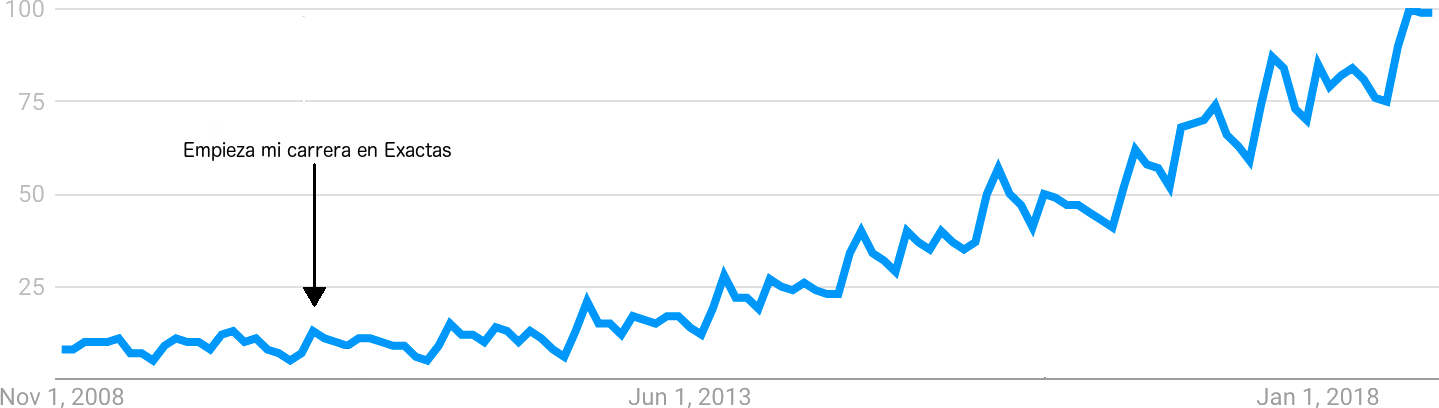
\includegraphics[width=\framewidth]{data_science_google_trends.png}
		\caption{Google trends for the term ``Data Science''\footcite{datasciencegt}}
	\end{figure}
	
\note{%
	En los últimos años hubo un crecimiento exponencial en la capacidad de acumular, guardar, y manipular cantidades masivas de datos sobre un gran espectro de disciplinas.

	Este crecimiento creó una pequeña revolución en muchas disciplinas académicas donde se solían usar encuestas u otros datos más particulares.
}
\end{frame}

\section{Marco Teórico}

\subsection{Homofilia Social}

\begin{frame}
	\epigraph{``La gente ama a los que son como sí mismos.''}{\textit{Aristoteles \\ Retórica}}
	\note{%
		La similaridad lleva a la conexión.

		La gente tiene características, como edad, género, o estatus socioeconómico, con el que hay una mayor tasa de contacto que gente disimilar.

		El trabajo hecho en esta tesis está relacionado a descubrir y explotar casos de homofilia en la población de un grafo social.
	}
\end{frame}

\begin{frame}
	\begin{figure}
		\begin{subfigure}[b]{0.48\framewidth}
			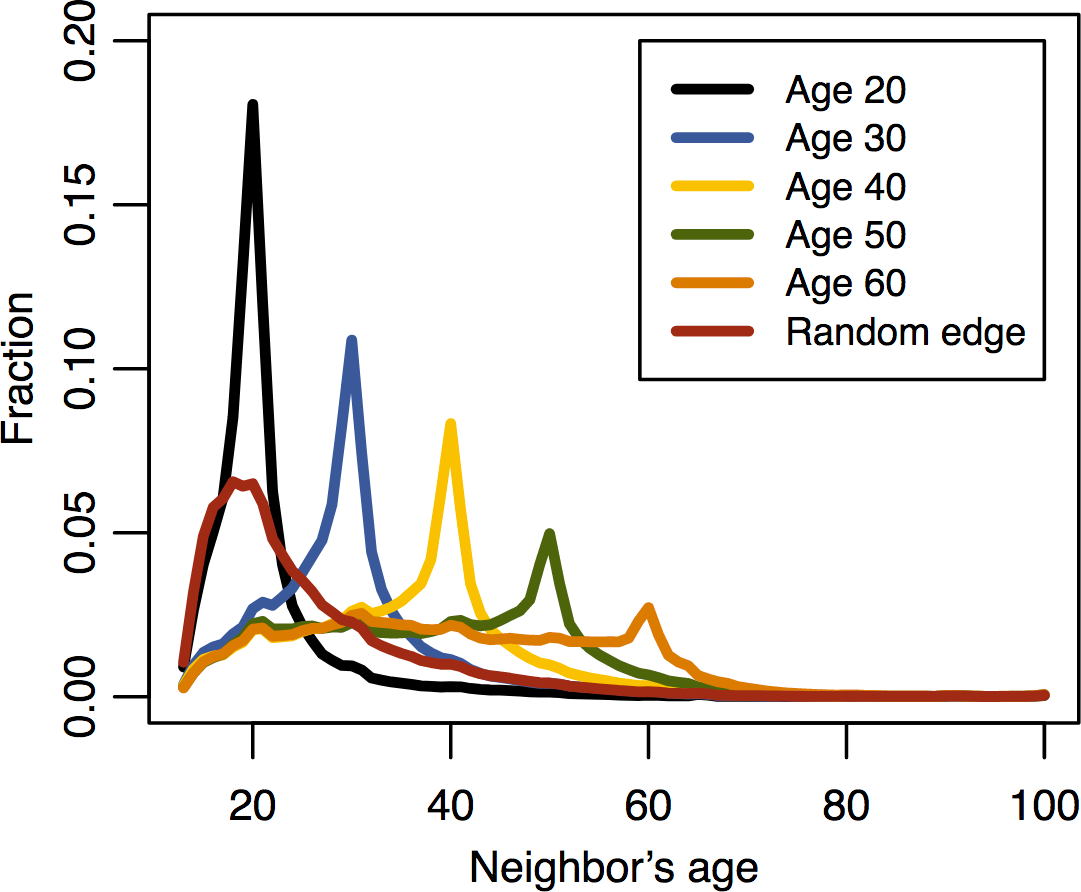
\includegraphics[width=0.9\textwidth]{age_homophily.png}
			\caption{}%
			\label{fig:age_homophily}
		\end{subfigure}
		\begin{subfigure}[b]{0.48\framewidth}
			\hfill{}
			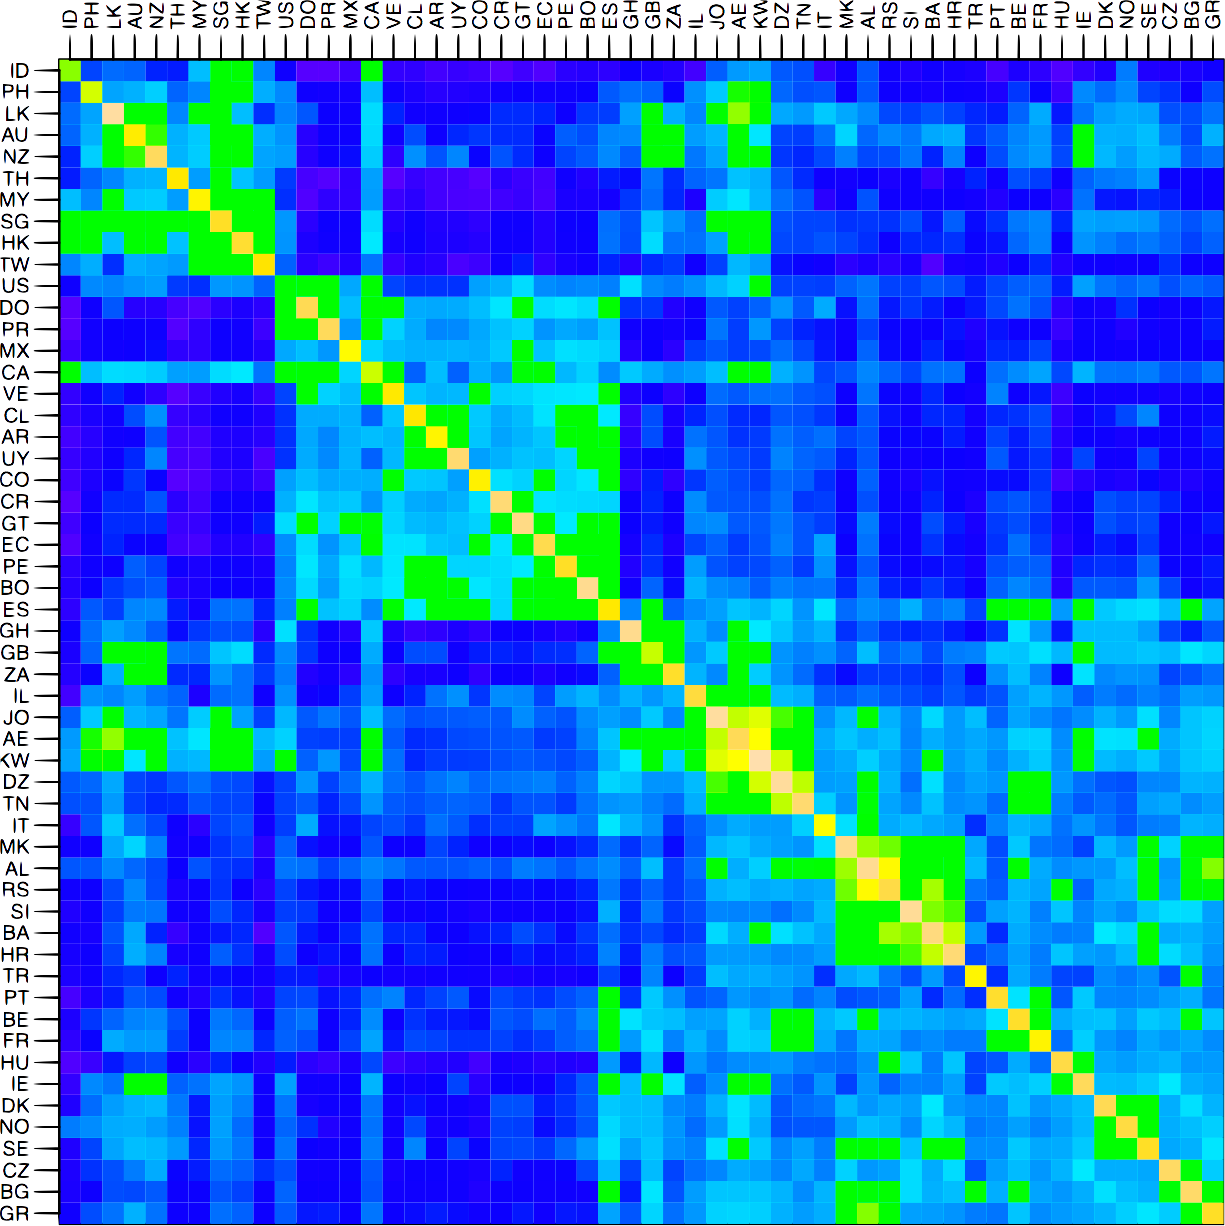
\includegraphics[width=0.9\textwidth]{country_homophily.png}
			\caption{}%
			\label{fig:country_homophily}
		\end{subfigure}
		\caption{Ejemplos varios de homofilia en un cierto grafo social\footcite{ugander2011anatomy}. \subref{fig:age_homophily}: Distribución de edades para contactos de usuarios de cada edad. \subref{fig:country_homophily}: Mapa de calor marcando la cantidad normalizada de contactos entre cada par de países.}
	\end{figure}

	\note{%
		Dos casos muy comunes de homofilia en grados sociales son la homofilia por edad y la homofilia por país. Ambas fueron investigadas por Ugander~et~al en el paper citado en este slide.

		Como se pueden apreciar en estos gráficos, el rango de edades para las conexiones de amistad en una red social están altamente sesgadas hacia la misma edad que tiene cada persona. También se puede ver lo mismo cuando se grafica los pares entre países entre todas las conexiones de amistad.
	}
\end{frame}

\subsection{Inferencia Bayesiana}

\begin{frame}{Inferencia Bayesiana}
	\parbox{.5\textwidth}{\raggedleft{}
		\begin{equation*}
			P \left( H \mid E \right) = \frac{P \left( E \mid H \right) \cdot P \left( H \right)}{P \left( E \right)}
		\label{eq:bayes}
		\end{equation*}
	}
	\hfill
	\parbox{.45\textwidth}{\raggedright{}
	\epigraph{``Dada la cantidad de veces en el que un evento desconocido sucedió y falló en suceder, la probabilidad de este pasando en una sola prueba está entre dos grados de probabilidad que pueden ser nombrados''}{\textit{Thomas Bayes \\ An Essay towards solving a Problem in the Doctrine of Changes}}
	}

	\note{%
		Parte de este trabajo usa enfoque bayesiano a las estadísticas. A diferencia del común enfoque frecuentista, donde los parámetros están fijos y desconocidos y las hipótesis son ciertas o falsas, cualquier cosa desconocida se describe con una distribución de probabilidad que describe su incertidumbre.
	}
\end{frame}

\subsection{Teorema de Bayes}

\begin{frame}{Teorema de Bayes}
	\begin{align*}
		&P \left( H \mid E \right) = \frac{P \left( E \mid H \right) \cdot P \left( H \right)}{P \left( E \right)} &\text{\textbf{Teorema de Bayes}} \\
		\vspace{4em} \\
		\onslide<1> {%
		&P \left( H \mid E \right) &\text{\textbf{Posterior Probability}} \\
		&P \left( E \mid H \right) &\text{\textbf{Likelihood}} \\
		&P \left( H \right) &\text{\textbf{Prior Probability}} \\
		&P \left( E \right) &\text{\textbf{Marginal Likelihood}}
		}
		\onslide<2> {%
			&P \left( H \mid E \right) \propto P \left( E \mid H \right) \cdot P \left( H \right) &\text{\textbf{Posterior Proportionality}}
		}
	\end{align*}
	
	\note{%
		\onslide<1>{%
			El teorema de Bayes describe la probabilidad de un evento en base a conocimiento a priori de las condiciones posiblemente relacionadas a este. Este tiene cuatro términos.
			\begin{itemize}
				\item \textbf{Posterior Probability}, que es la probabilidad condicional asignada después de que el evento se toma en cuenta. \\
				\item \textbf{Likelihood}, el grado de probabilidad de $E$ dado que $H$ es cierto. \\
				\item \textbf{Prior Probability}, las suposiciones hechas en el problema antes de los experimentos. \\
				\item \textbf{Marginal Likelihood}, la función de probabilidad donde algunos parámetros fueron marginalizados. Se usa como constante normalizante para que la \emph{Posterior Probability} integre a $1$, haciendo que sea una probabilidad válida.
			\end{itemize}
		}
		\onslide<2>{%
			Estas ecuaciones son probabilidadeso continuas, que por definición deben integrar a $1$. Por esa razón, se suele usar la ecuación en este \textit{slide}, que define la proporcionalidad del \textit{posterior}.
		}
	}
\end{frame}

\subsection{Distribución Beta}

\begin{frame}{Distribución Beta}
	\begin{align*}
		X &\sim B \left( \alpha, \beta \right) \\
		\mathrm{B} \left( \alpha, \beta \right) &= \frac{\left( \alpha + \beta - 1 \right)!}{\left( \alpha - 1 \right)! \cdot \left( \beta - 1 \right)!}
	\vspace{1em} \\
		f \left( X; \alpha, \beta \right) &= \frac{1}{\mathrm{B} \left(\alpha, \beta \right)} \cdot x^{\alpha - 1} {\left( 1 - x \right)}^{\beta - 1} \\
		\vspace{1em} \\
		F \left( X; \alpha, \beta \right) &= P \left( X \leq x \right) \\
		F \left( X; \alpha, \beta \right) &= \frac{1}{\mathrm{B} \left(\alpha, \beta \right)} \cdot \int^x_0 {t^{\alpha - 1} {\left( 1 - t \right)}^{\beta - 1} dt} \\
		\vspace{1em} \\
		Q \left( p \right) &= \inf \left\{ x \in \mathbb{R} \mid p \leq F \left( x \right) \right\}
	\end{align*}

	\note{%
		La distribución Beta es una familia de distribuciones de probabilidad paramterizada por dos parámetros $\alpha$ y $\beta$. Se suele usar para modelar como actúan variables aleatorias limitadas a intervalos de largo finito.

		En el contexto de inferencia bayesiana, la distribución Beta es el conjugate prior de la distribución binomial. Esto nos permite describir conocimientos iniciales sobre la probabilidad de éxito de una distribución bivariada.

		Dado una distribución binomial con $\alpha$ ejemplos positivos y $\beta$ ejemplos negativos como tirar una moneda $(\alpha + \beta)$ veces, la distribución Beta modela la probabilidad de que la primer distribución sea positiva.
		
		El trabajo principal de esta tesis usa mucho la función cuántil de la distribución Beta, que es la inversa de la función cumulativa de probabilidad. No hay ninguna formula cerrada para esto, pero se puede aproximar fácilmente usando el método de Newton.
	}
\end{frame}

\begin{frame}{Distribución Beta}
	
	\begin{figure}
		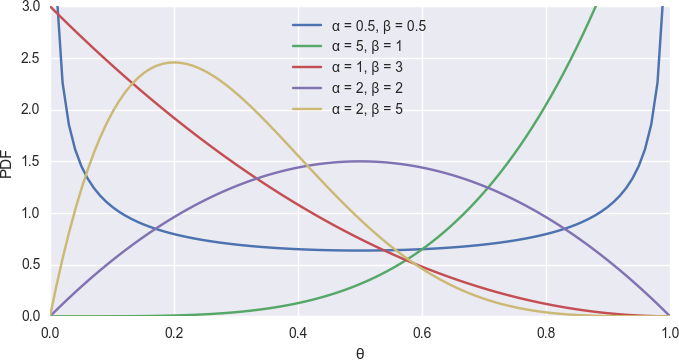
\includegraphics[width=\framewidth]{beta.png}
		\caption{Distribución Beta para diferentes valores de $\alpha$ y $\beta$.}
	\end{figure}
	
	\note{%
		Este gráfico representa la distribución Beta para diferentes valores de $\alpha$ y $\beta$.
	}
\end{frame}

\section{Fuente de Datos}

\subsection{Fuente de Datos}

\begin{frame}{Fuente de Datos}
	\begin{itemize}
		\item Esta tesis usa dos fuentes de datos principales para cierta población.
			\begin{enumerate}
				\item Dos conjuntos $P$ y $S$ con \emph{Call Detail Records} de llamadas y SMS\@.
				\item Un conjunto $B$ de datos bancarios, del cual se puede extraer el salario mensual.
			\end{enumerate}
		\item Con estos datos se calcula el \emph{Grafo Social}.
			\begin{equation*}
				G = \left< \text{V}, \text{E} \right>
			\end{equation*}
			Donde $V$ contiene datos de usuarios y su nivel de ingreso (si se conoce), y $E$ contiene sus conexiones con otros usuarios.
	\end{itemize}
\end{frame}

\subsection{Inferencias Básicas}
\begin{frame}{Distribución de Ingresos por Edad}
	\begin{figure}
		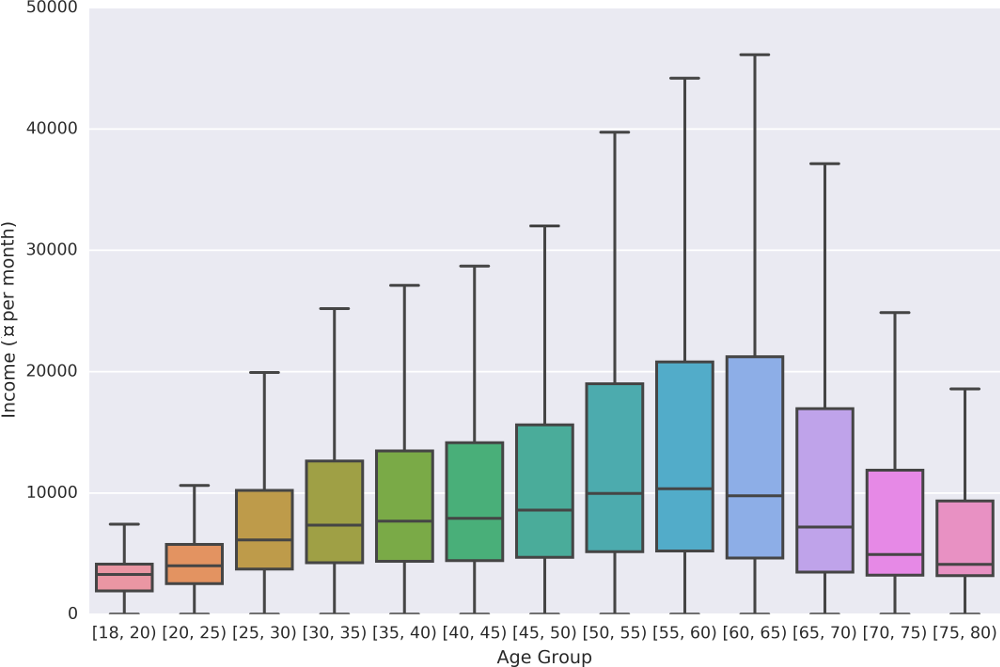
\includegraphics[width=.80\framewidth]{income_age_boxplot4.png}
		\caption{Distribución de ingresos por grupo de edad.}
	\end{figure}
\end{frame}

\begin{frame}{Distribución de Ingresos Totales}
	\parbox{.60\textwidth}{\raggedleft{}
		\begin{figure}
			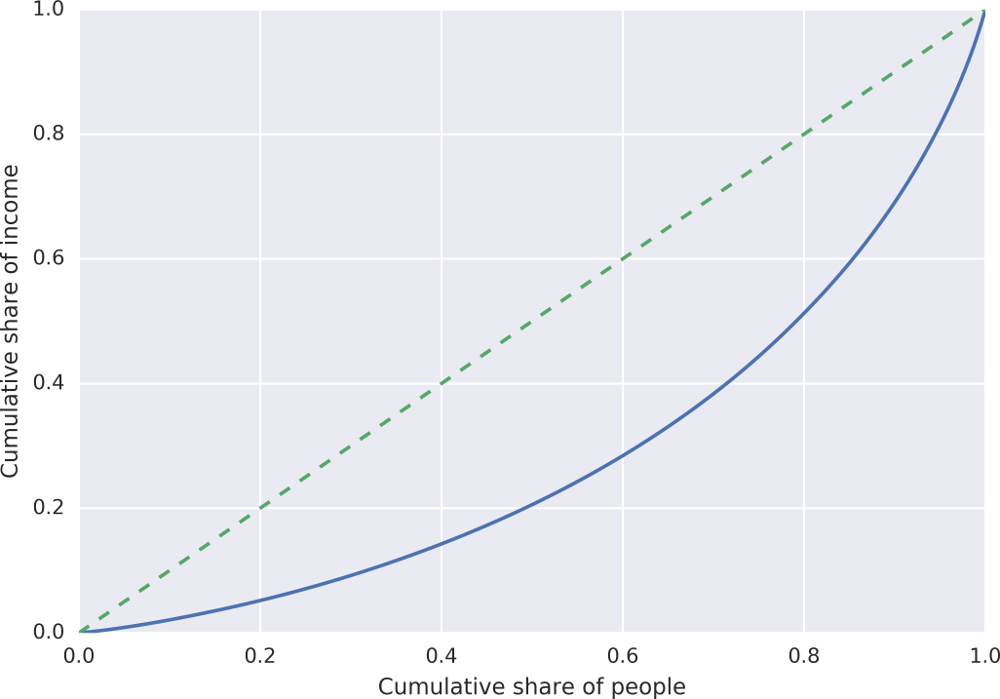
\includegraphics[width=.6\framewidth]{cumulative_income.png}
			\caption{Proporción acumulada de ingresos por proporción acumulada de la población.}
		\end{figure}
	}
	\parbox{.39\textwidth}{\raggedright{}
		Dentro de los usuarios de este banco:
		\begin{itemize}
			\item 20\% de la población tiene 50\% de los activos.
			\item Gini = 45\%.
		\end{itemize}
	}

	\note{%
		Este gráfico nota la desigual distribución de ingresos dentro de los usuarios del banco, donde la mayoría de los activos líquidos pertenecen a menos de un quinto de la población.

		El coeficiente Gini mide la desigualdad de riqueza de un grupo de gente: un valor de 0\% indica total igualdad, mientras que un valor de 100\% indica una sola persona teniendo toda la riqueza. El coeficiente en este banco es igual a 45\%, que es un poco menor al valor total de 48\% del país del estudio ya que no incluye a la población no bancarizada de este país.
	}
\end{frame}

\section{El Modelo Bayesiano}

\subsection{Introducción}

\begin{frame}{Introducción}
	El objetivo principal de esta tesis es buscar un algoritmo que prediga el nivel de ingresos de un usuario dependiendo de datos sobre el \emph{Grafo Social}.

	Esto se logra aprovechando el nivel de \emph{Homofilia de Ingresos} en los usuarios.
\end{frame}


\subsection{Homofilia de Ingresos}

\begin{frame}{Coeficiente de Spearman}
	El Coeficiente de Spearman $r_s$ mide la correlación entre la distribución de dos monotónicas variables $x$ e $y$~\footcite{statistical_analysis}, donde $\rho_{x, y}$ es el \emph{Coeficiente de Pearson} entre $x$ e $y$.


	\begin{equation*}
		r_s = \rho_{\rank\left(x\right), \rank\left(y\right)} = \frac{\cov\left(\rank\left(x\right), \rank\left(y\right))}{\sigma_{\rank(x)} \sigma_{\rank(y)}}
	\end{equation*}

	\onslide<2>{%
		\vspace{2em} \\

		En la fuente de datos usada para esta tesis,

		\begin{equation*}
			r_s = 0.474
		\end{equation*}
	}
\end{frame}

\begin{frame}
	\begin{figure}
		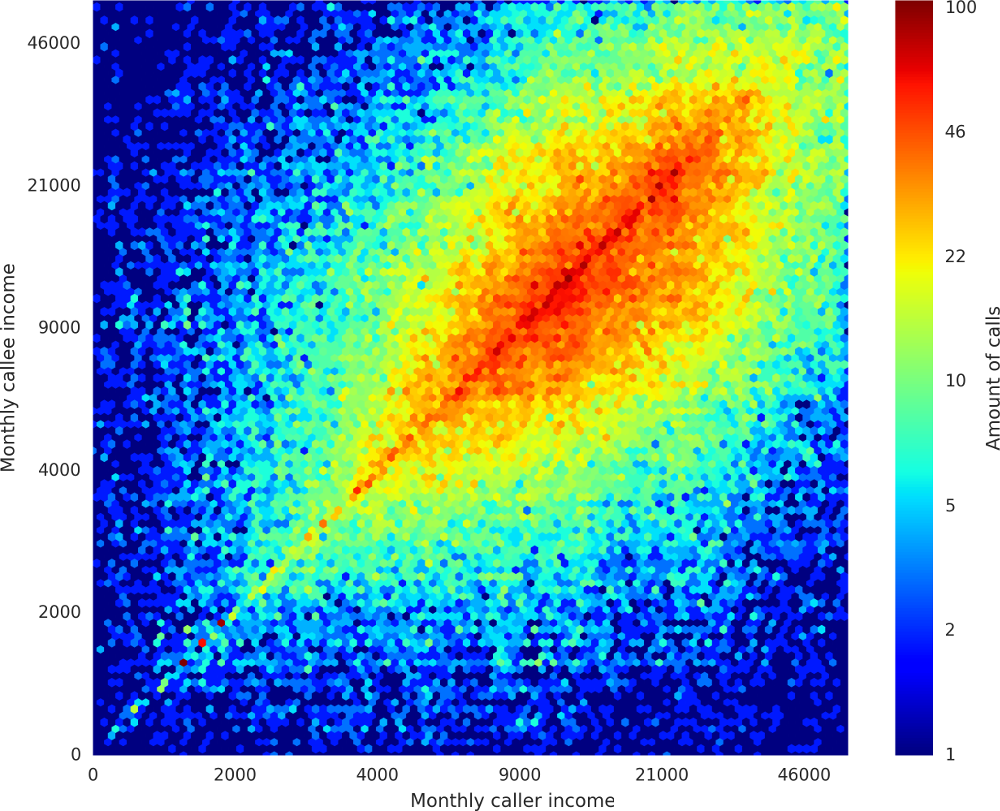
\includegraphics[width=.8\framewidth]{heatmap.png}
		\caption{Mapa de calor entre ingresos de usuarios de cada llamada.}
	\end{figure}
\end{frame}

\subsection{El Modelo Bayesiano}

\begin{frame}{El Modelo Bayesiano}
	
	\note{%
		La principal contribución de esta tesis es un modelo bayesiano de predicción de nivel de ingresos para los usuarios del grafo social y encontrar usuarios de altos ingresos.
	}
\end{frame}

\begin{frame}{El Modelo Bayesiano}
	\begin{align*}
		H_1 &= \left\{ v \mid v \in V \wedge v_s \leq 6300 \right\} &\text{Usuarios de \emph{Bajos Ingresos}} \\
		H_2 &= \left\{ v \mid v \in V \wedge v_s >    6300 \right\} &\text{Usuarios de \emph{Altos Ingresos}}
	\end{align*}
\end{frame}

\begin{frame}{El Modelo Bayesiano}
	\begin{gather*}
		\begin{aligned}
			& \calls^{\low}_v = \sum_{\substack{e \in E \\ e_d = v \\ e_o \in H_1}}{e_c} + \sum_{\substack{e \in E \\ e_o = v \\ e_d \in H_1}}{e_c}
			& \calls^{\high}_v = \sum_{\substack{e \in E \\ e_d = v \\ e_o \in H_2}}{e_c} + \sum_{\substack{e \in E \\ e_o = v \\ e_d \in H_2}}{e_c} \\
			& \etime^{\low}_v = \sum_{\substack{e \in E \\ e_d = v \\ e_o \in H_1}}{e_t} + \sum_{\substack{e \in E \\ e_o = v \\ e_d \in H_1}}{e_t}
			& \etime^{\high}_v = \sum_{\substack{e \in E \\ e_d = v \\ e_o \in H_2}}{e_t} + \sum_{\substack{e \in E \\ e_o = v \\ e_d \in H_2}}{e_t} \\
			& \sms^{\low}_v = \sum_{\substack{e \in E \\ e_d = v \\ e_o \in H_1}}{e_s} + \sum_{\substack{e \in E \\ e_o = v \\ e_d \in H_1}}{e_s}
			& \sms^{\high}_v = \sum_{\substack{e \in E \\ e_d = v \\ e_o \in H_2}}{e_s} + \sum_{\substack{e \in E \\ e_o = v \\ e_d \in H_2}}{e_s}
		\end{aligned} \\
		\vspace{1em} \\
		\begin{aligned}
			\contacts^{\low}_v &= &\left| \left\{ e \in E \mid e_o = v \land e_d \in H_1 \right\} \cup \left\{ e \in E \mid e_d = v \land e_o \in H_1 \right\} \right| \\
			\contacts^{\high}_v &= &\left| \left\{ e \in E \mid e_o = v \land e_d \in H_2 \right\} \cup \left\{ e \in E \mid e_d = v \land e_o \in H_2 \right\} \right|
		\end{aligned}
	\end{gather*}
\end{frame}

\begin{frame}{El Modelo Bayesiano}
	\begin{equation*}
		\varpi \in \left\{ \calls, \etime, \sms, \contacts \right\}
	\end{equation*}
\end{frame}

\begin{frame}{El Modelo \sout{Bayesiano} Frecuentista}
	\onslide<1->{%
	\begin{equation*}
		p_v = P \left( v \in H_2 \right) = \frac{\varpi^{\high}_v}{\varpi^{\high}_v + \varpi^{low}_v}
	\end{equation*}
	}

	\onslide<2->{%
		Dados $a$ y $b$ donde
		
		\begin{gather*}
			\begin{aligned}
				&\calls^{\high}_a = 1   &\calls^{\low}_a = 0 \\
				&\calls^{\high}_b = 100 &\calls^{low}_b = 1
			\end{aligned} \\
			\vspace{1em} \\
			p_a > p_b
		\end{gather*}
	}

	\note{%
		Este modelo parece obviamente correcto, pero no modela la \emph{Incertidumbre} por la falta de información de dos usuarios
	}
\end{frame}

\begin{frame}{El Modelo Bayesiano}
	Se define una distribución Beta diferente para cada usuario $v \in V$.

	\begin{gather*}
		\Betasim_v \sim B \left( \varpi^{\high}_v + 1, \varpi^{\low} + 1 \right) \\
		\onslide<2-> {%
		P \left( \Betasim_v \leq x \right) = \frac{1}{B \left( \varpi^{\high} + 1, \varpi^{\low} + 1 \right)} \cdot \int^x_0 {t^{\varpi^{\high}_v} {\left( 1 - t \right)}^{\varpi^{\low}_v} dt}
		}
	\end{gather*}
	
	\onslide<3->{%
		Para medir la \emph{Incertidumbre}, se elige un cuántil arbitrario $\Theta \in \left[ 0, 1 \right]$ y se define
		\begin{align*}
			p_v &= Q \left( \Theta \right) \\
			&= \inf \left\{ x \in \left[ 0, 1 \right] \mid \Theta \leq F \left( x \right) \right\}
		\end{align*}

		Esta representa la \emph{posterior probability} de $p_v$ dados los datos.
	}
\end{frame}

\begin{frame}{El Modelo Bayesiano}
	\onslide<1->{%
		\begin{equation*}
			p_v &= Q \left( \Theta \right)
		\end{equation*}
	}
	\onslide<1>{%
		Dados dos usuarios $v$ y $u$, $p_v > p_u$ implica que $v$ tiene mayor probabilidad de tener altos ingresos que $u$.

		Si $u$ tiene altos ingresos y $p_v > p_u$, $v$ tiene altos ingresos.
	}
	\onslide<2->{%
		\begin{gather*}
			\tau \in \left[ 0, 1 \right]  \\
			\vspace{1em} \\
			\begin{aligned}
				p_v \leq \tau &\implies v \in H_1 \\
				p_v >    \tau &\implies v \in H_2
			\end{aligned}
		\end{gather*}

		$\tau$ representa el umbral (threshold) que el algoritmo usa para separar usuarios de bajos y altos ingresos. Este valor puede usarse para incrementar o decrementar la precisión del modelo a cambio de recall.
	}
\end{frame}

\subsection{Evaluación del Modelo}

\begin{frame}{Evaluación del Modelo}
	\begin{itemize}
		\item $B$ Usuarios del banco.
		\pause{}
		\item $B_{\train}$ \emph{Training set} base.
		\item $B_{\test}$ \emph{Testing set} base.
			\begin{gather*}
				B = B_{\train} \cup B_{\test} \\
				\left| B_{\train} \right| = 0.8 \cdot \left|B| \qquad
				\left| B_{\test} \right| = 0.2 \cdot \left|B|
			\end{gather*}
		\pause{}
		\item $\hat{E}$ Usuarios con un algún vecino en el \emph{training set}.
		\item $\hat{B}_{\test}$ Usuarios del \emph{testing set} con algún vecino en el \emph{training set}.
			\begin{gather*}
				\hat{E} = \left\{ e \in E \mid e_o \in B_{\train} \lor e_d \in B_{\train} \right\} \\
				\hat{B}_{\test} = B_{\test} \cap \left( \hat{E}_o \cup \hat{E}_d \right)
			\end{gather*}
		\pause{}
		\item $\Upsilon$ Usuarios en $\hat{B}_{\test}$ con los labels balanceados.
			\begin{equation*}
				\left| \Upsilon_{\low} \right| = \left| \Upsilon_{\high} \right|
			\end{equation*}
	\end{itemize}
\end{frame}

\subsection{Optimizando $\Theta$}

\begin{frame}{Optimizando $\Theta$}
	Para medir la \emph{Incertidumbre}, se elige un cuántil arbitrario $\Theta \in \left[ 0, 1 \right]$ y se define
	\begin{align*}
		p_v &= Q \left( \Theta \right) \\
		&= \inf \left\{ x \in \left[ 0, 1 \right] \mid \Theta \leq F \left( x \right) \right\}
	\end{align*}

	Esta representa la \emph{posterior probability} de $p_v$ dados los datos.
\end{frame}

\begin{frame}{Optimizando $\Theta$}
	\begin{figure}
		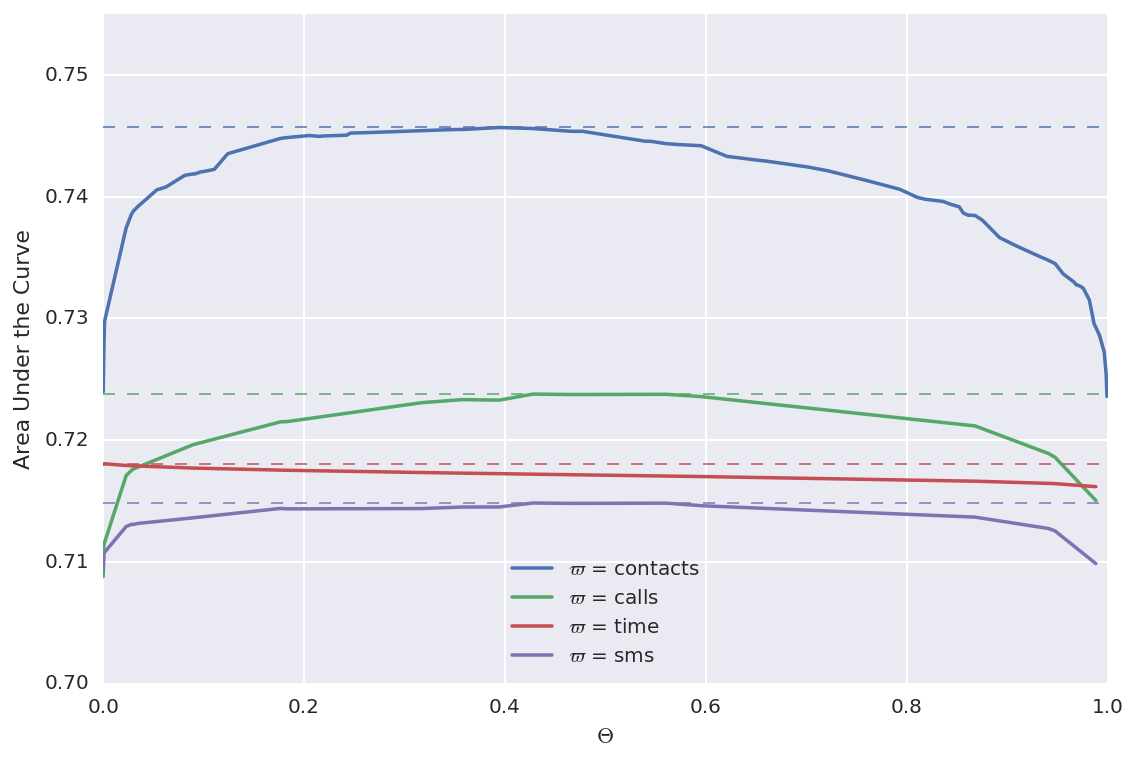
\includegraphics[height=.75\textheight]{theta.png}
		\caption{El \emph{área bajo la curva} del modelo bayesiano para diferentes $\varpi$ en base a $\Theta$.}
	\end{figure}
\end{frame}

\begin{frame}{Optimizando $\Theta$}
	\begin{table}
		\centering
		\begin{tabular}{l r r}
			$\varpi$ & $\Theta$ Óptimo & AUC \\
			contacts & \num{0.394} & \num{0.746} \\
			calls & \num{0.428} & \num{0.724} \\
			time & \num{0.001} & \num{0.718} \\
			sms & \num{0.428} & \num{0.715}
		\end{tabular}
		\caption{Resultados para $\Theta$ que maximizan el \emph{área bajo la curva}.}
	\end{table}
\end{frame}

\subsection{Optimizando $\tau$}

\begin{frame}{Optimizando $\tau$}
	\begin{itemize}
		\item Eligiendo un $\varpi$ y dado un $\Theta$, ya tenemos un buen modelo de predicción para $p_v$, la probabilidad de que $v$ sea un usuario de altos ingresos.
		\item $\tau$ representa el umbral (threshold) que el algoritmo usa para separar usuarios de bajos y altos ingresos.
			\begin{gather*}
				\begin{aligned}
					p_v \leq \tau &\implies v \in H_1 \\
					p_v >    \tau &\implies v \in H_2
				\end{aligned}
			\end{gather*}
		\item Para cada $\varpi$, se elige el $\tau$ que maximice la \emph{exactitud} (accuracy) del modelo.
	\end{itemize}
\end{frame}

\begin{frame}{Infiriendo por Cantidad de Llamadas}
		\begin{figure}
			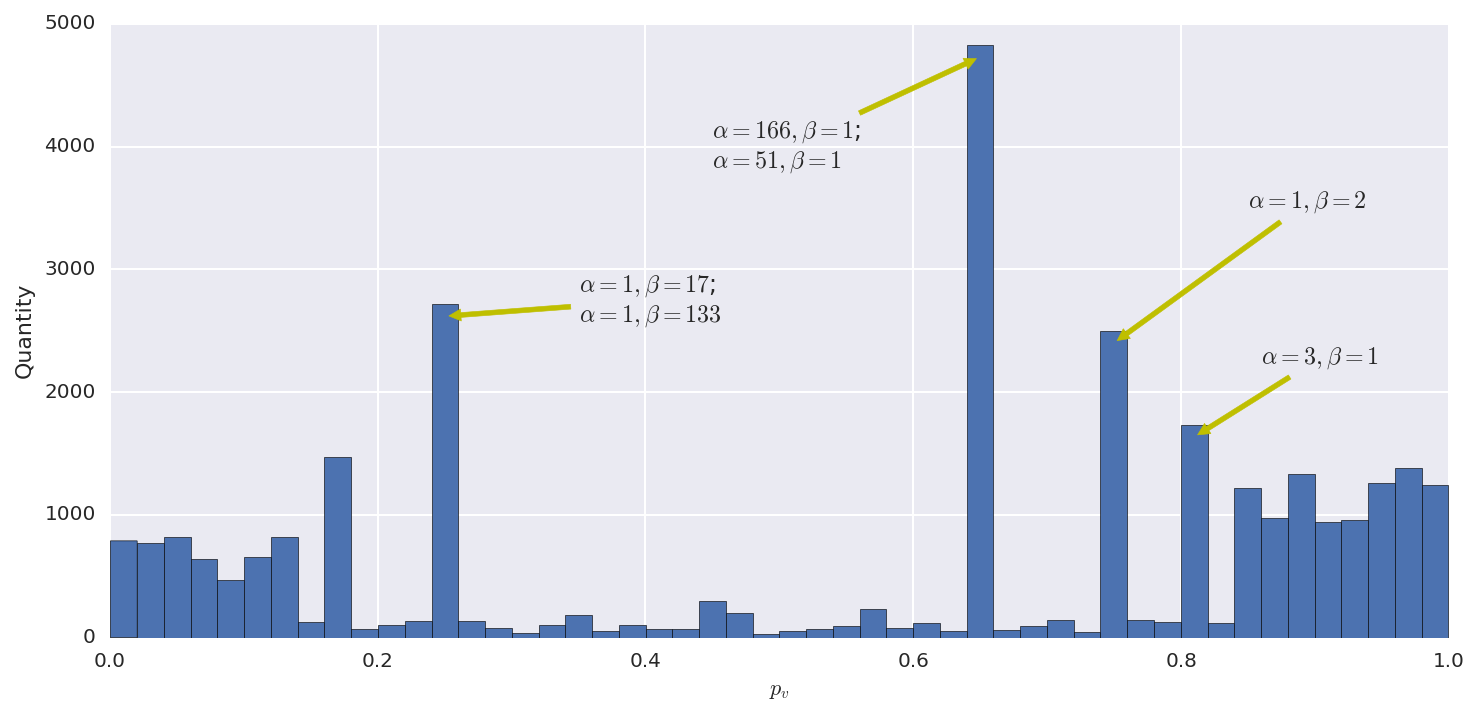
\includegraphics[width=\framewidth, height=.37\textheight, keepaspectratio]{figures/bayes/hist_calls.png} \\
			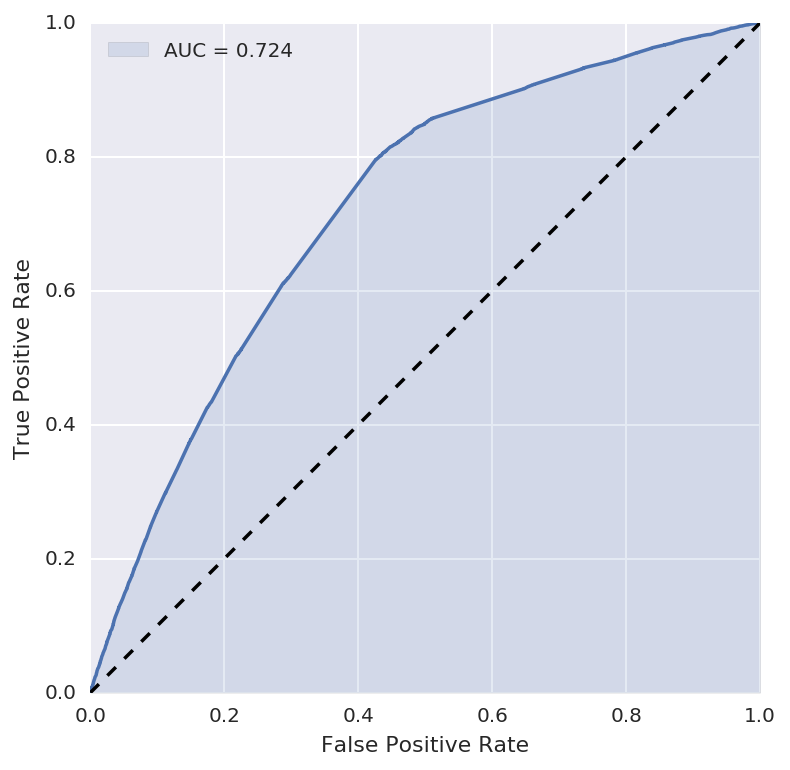
\includegraphics[width=.49\framewidth, height=.37\textheight, keepaspectratio]{figures/bayes/roc_calls.png}
			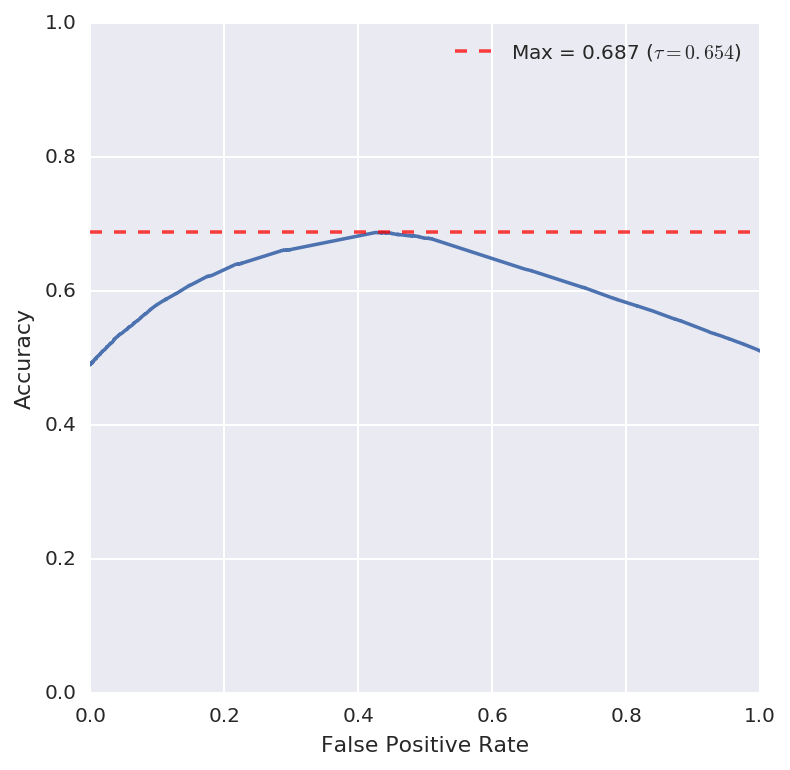
\includegraphics[width=.49\framewidth, height=.37\textheight, keepaspectratio]{figures/bayes/accuracy_calls.png}
			\caption{Resultados del \emph{método bayesiano} usando cantidad de llamados. $\tau = 0.654$}
		\end{figure}

		\note{%
			\Cref{fig:bayes_calls} contains data about the predictor when $\varpi = \calls$ and the data is analyzed using $\Upsilon^{\calls}$ as \emph{Testing Set}. The \emph{Inverse Cumulative Distribution Function} contains a few peaks for users with a similar amount of calls.

			After analyzing the data, we find that the \emph{Area Under the Curve} using this method is of \num{0.724}, which is significantly higher than all the naïve and \emph{Machine Learning} methods that will be presented in the later \cref{sec:comparison}.

			Setting $\tau = 0.654$ maximizes the accuracy at $\Accuracy = 0.687$. Additionally, that value of $\tau$ results in $\Precision = 0.653$, $\Recall = 0.815$, $F_1 = 0.725$, and $F_4 = 0.804$.
			}
\end{frame}

\begin{frame}{Infiriendo por Tiempo Total de Llamadas}

	\begin{figure}
		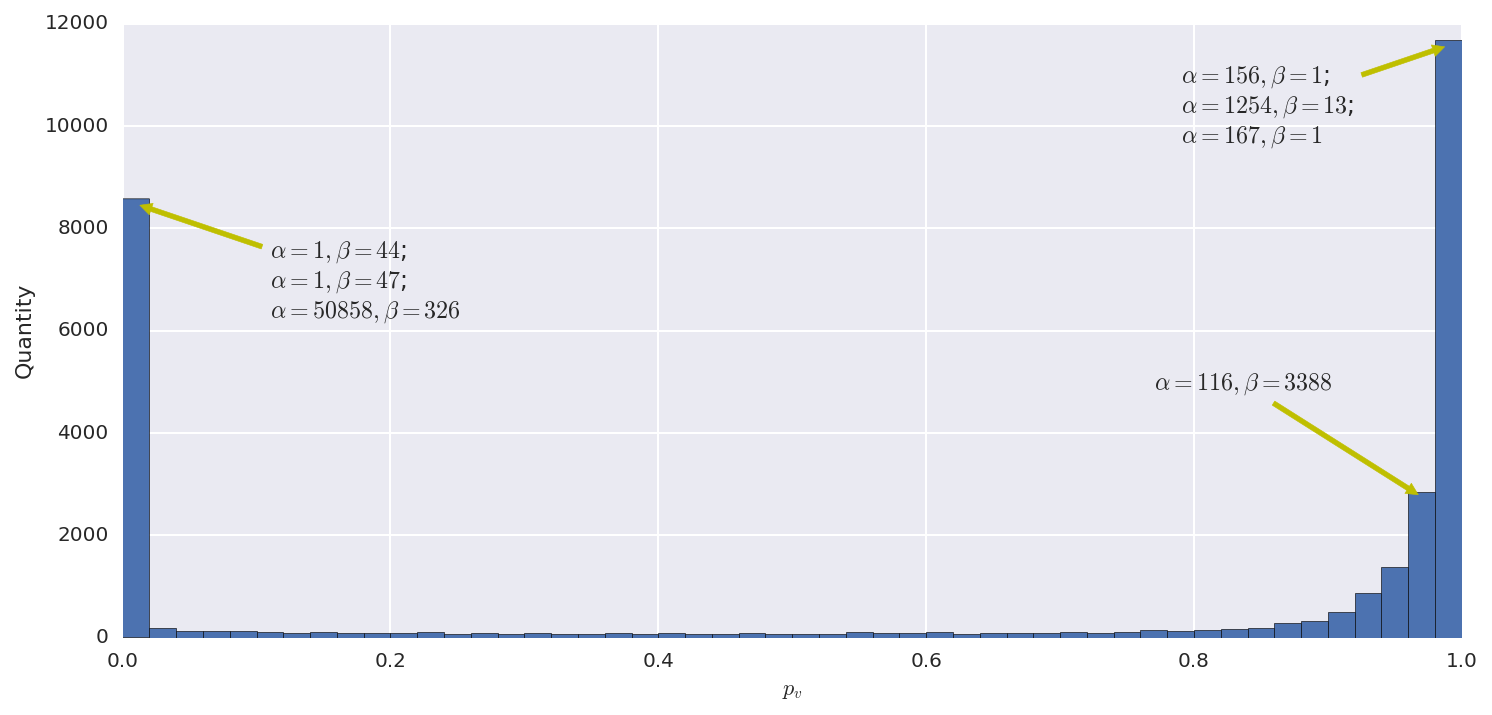
\includegraphics[width=\framewidth, height=.37\textheight, keepaspectratio]{figures/bayes/hist_time.png} \\
		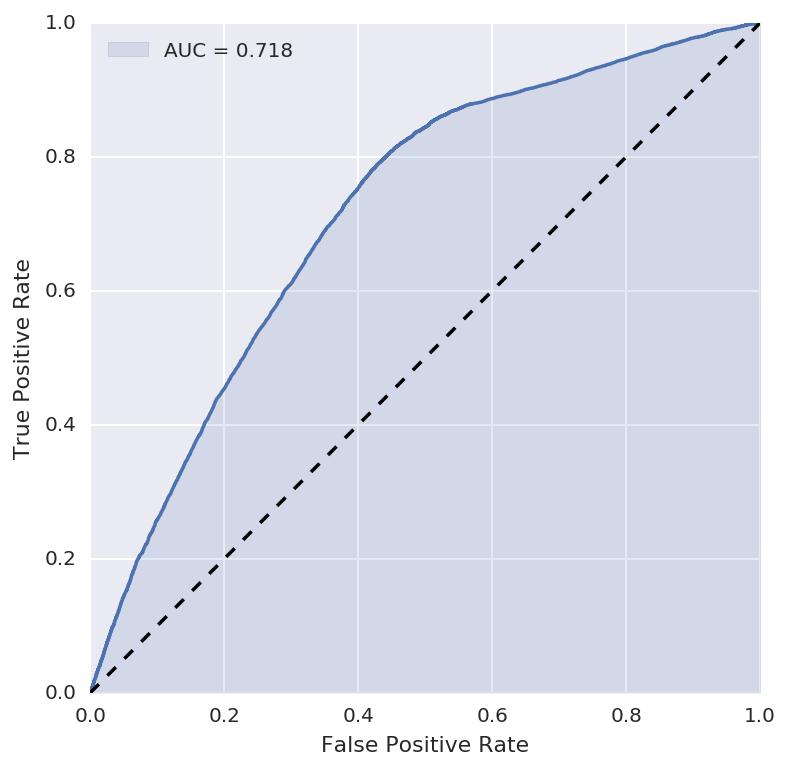
\includegraphics[width=.49\framewidth, height=.37\textheight, keepaspectratio]{figures/bayes/roc_time.png}
		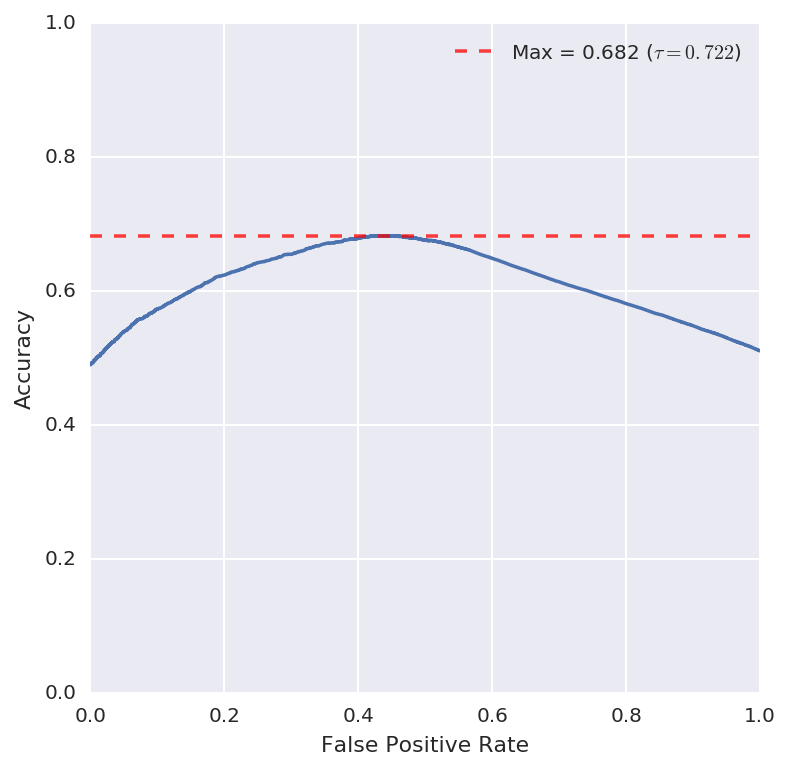
\includegraphics[width=.49\framewidth, height=.37\textheight, keepaspectratio]{figures/bayes/accuracy_time.png}
		\caption{Resultados del \emph{método bayesiano} usando tiempo total de llamads. $\tau = 0.722$}
	\end{figure}

\note{%
	\Cref{fig:bayes_time} contains data about the predictor when $\varpi = \etime$ and the data is analyzed using $\Upsilon^{\calls}$ as \emph{Testing Set}, there are two big clusters of data at the edges; this is explained because the majority of users spend most of their time talking to either \emph{High Income} or \emph{Low Income} users.

	The \emph{Area Under the Curve} of this inference mechanism is $\AUC = 0.718$, which is lower than the one for the calls in \cref{subsec:calls_infer}. The \emph{Accuracy Curve} is unsurprisingly similar to that one, and even the \emph{Accuracy} at $\tau = 0.722$ is the close. This is probably a result of the fact that there is an obvious correlation between total talking time and total calls.

	This $\tau$ also results in a predictor where $\Accuracy = 0.682$, $\Precision = 0.649$, $\Recall = 0.819$, $F_1 = 0.724$, and $F_4 = 0.807$.
}

\end{frame}

\begin{frame}{Infiriendo por Cantidad Total de Mensajes de Texto}

	\begin{figure}
		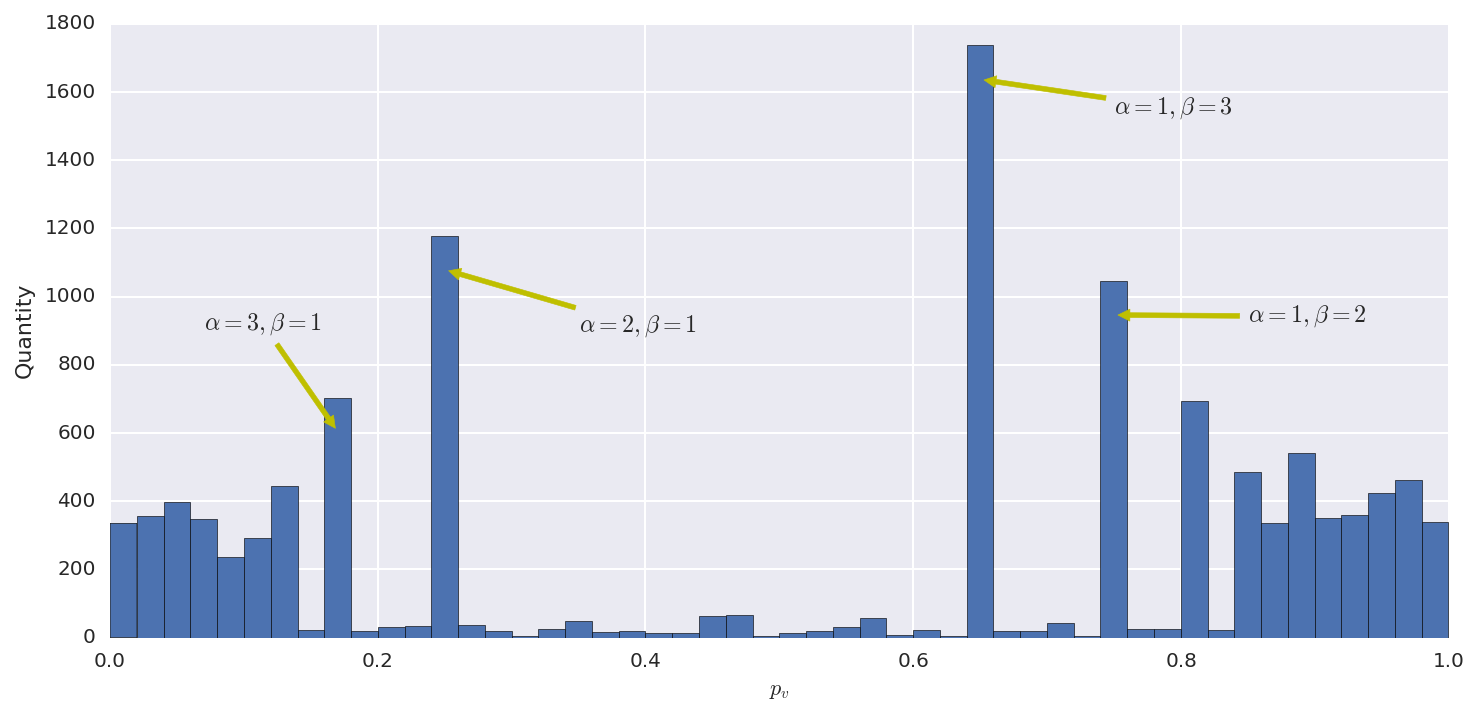
\includegraphics[width=\framewidth, height=.37\textheight, keepaspectratio]{figures/bayes/hist_sms.png} \\
		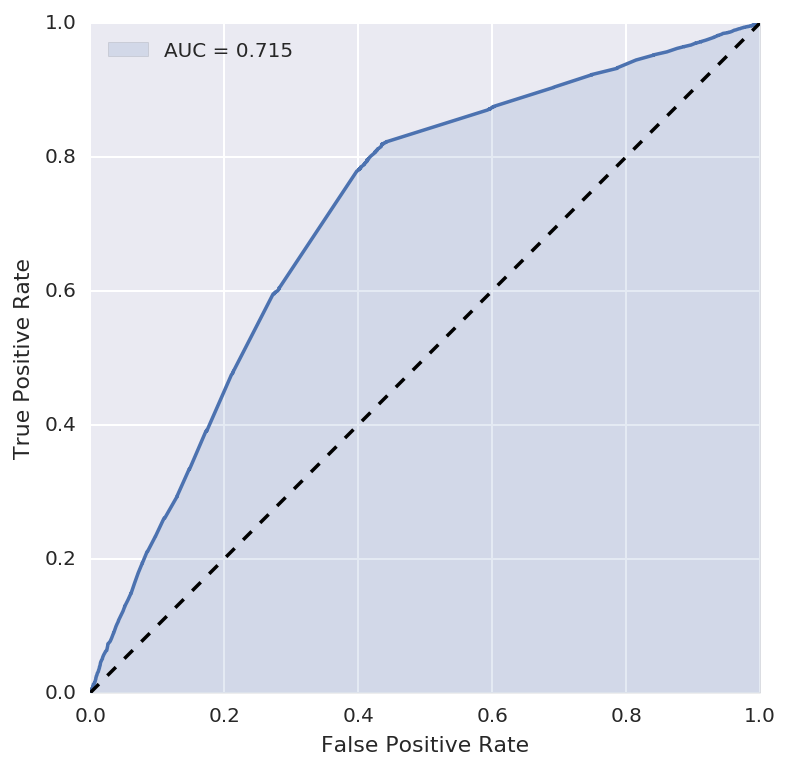
\includegraphics[width=.49\framewidth, height=.37\textheight, keepaspectratio]{figures/bayes/roc_sms.png}
		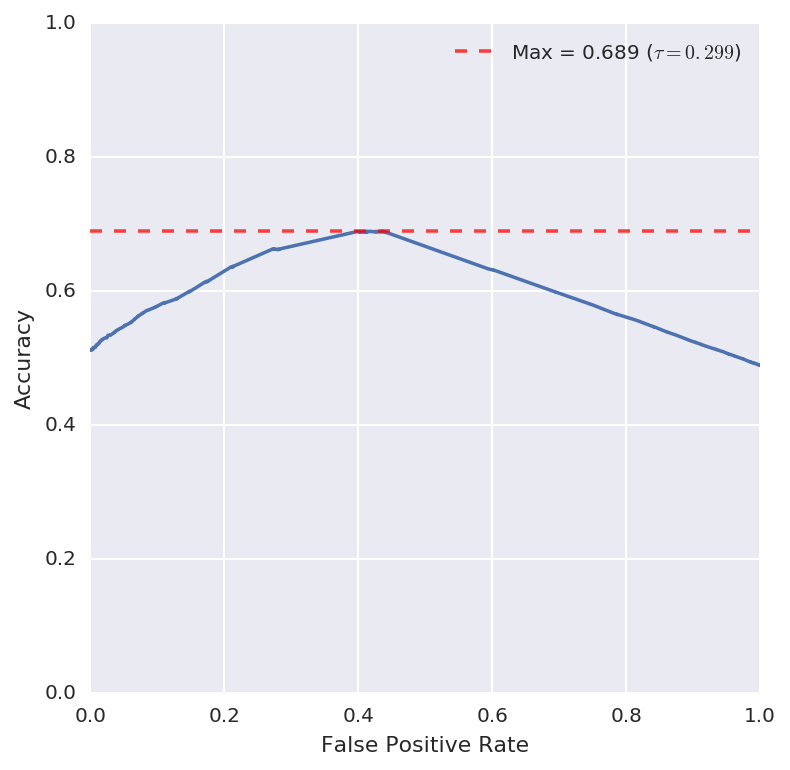
\includegraphics[width=.49\framewidth, height=.37\textheight, keepaspectratio]{figures/bayes/accuracy_sms.png}
	\caption{Resultados del \emph{método bayesiano} usando cantidad total de mensajes de texto. $\tau = 0.299$}
	\end{figure}

	\note{%
		\Cref{fig:bayes_sms} shows the distributions when $\varpi = \sms$. Since the total amount of SMS is much lower than the amount of calls, the peaks of the result of the \emph{Inverse Cumulative Functions} of the \emph{Beta Distribution} applied on $\Upsilon^{\sms}$ that happen with the majority of users that have few of both are located closer to the center than in \cref{subsec:calls_infer,subsec:time_infer}. This makes some interesting cases if $\varpi = \sms$ is chosen, since the distribution is different than in the other cases.

		In particular, this gives an $\AUC = 0.715$, which is lower than both in the case of \emph{Calls} and \emph{Time}. Interestingly, the maximum \emph{Accuracy} at $\tau = 0.299$ is slightly higher than both of the other cases; this is probably a side-effect of the fact that $\left| \Upsilon^{\sms} \right| < \left| \Upsilon^{\calls} \right|$.

		Additionally, $\Precision = 0.696$, $\Recall = 0.186$, $F_1 = 0.293$, and $F_4 = 0.194$.
	}

\end{frame}

\begin{frame}{Infiriendo por Cantidad de Contactos}

	\begin{figure}
		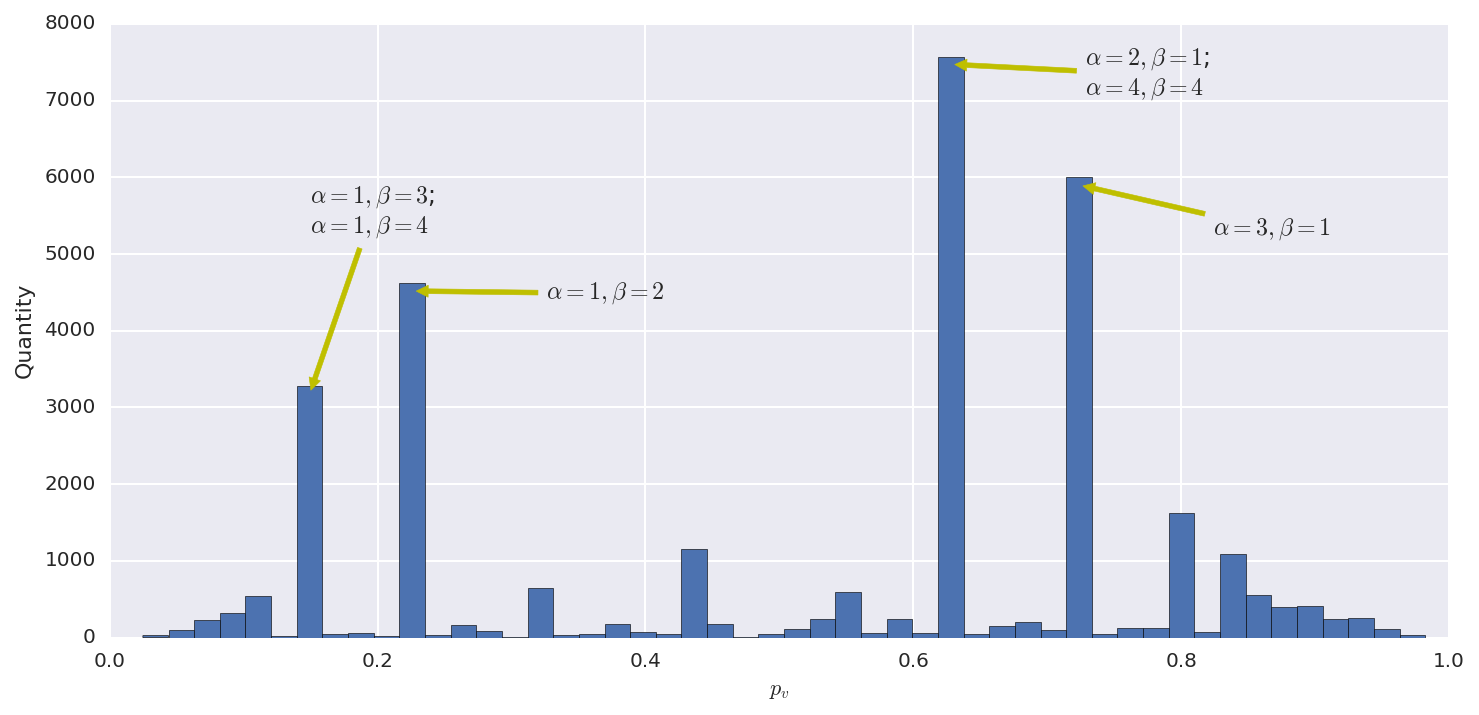
\includegraphics[width=\framewidth, height=.37\textheight, keepaspectratio]{figures/bayes/hist_contacts.png} \\
		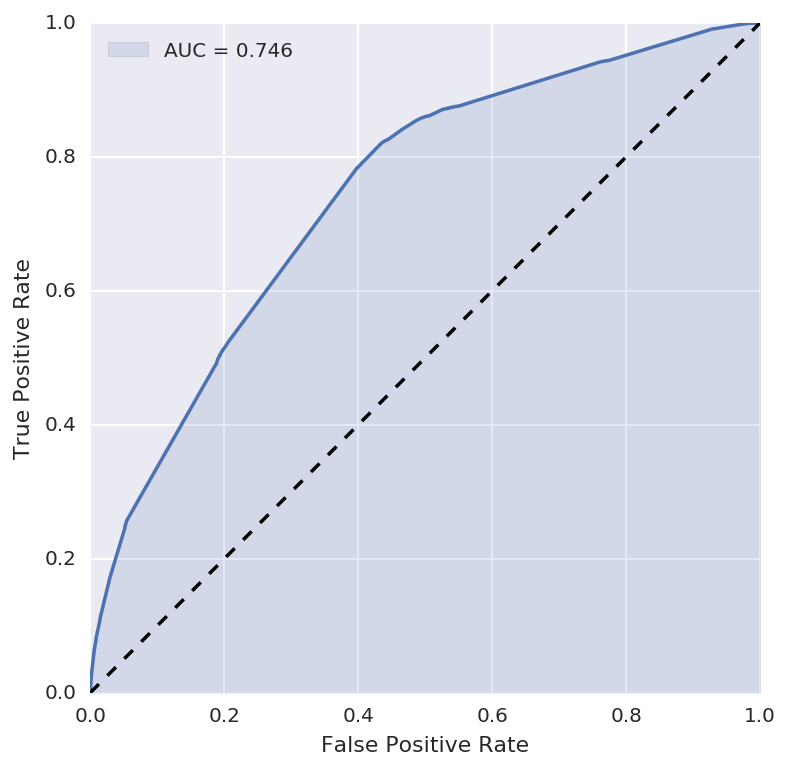
\includegraphics[width=.49\framewidth, height=.37\textheight, keepaspectratio]{figures/bayes/roc_contacts.png}
		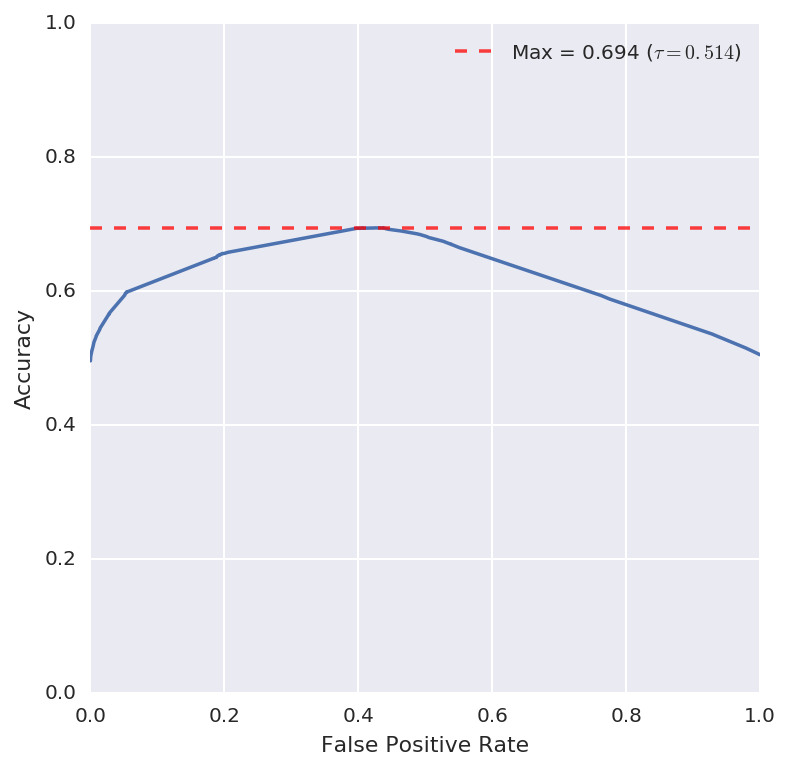
\includegraphics[width=.49\framewidth, height=.37\textheight, keepaspectratio]{figures/bayes/accuracy_contacts.png}

		\caption{Resultados del \emph{método bayesiano} usando el grado de cada usuario. $\tau = 0.514$}
	\end{figure}

	\note{%
		\Cref{fig:bayes_contacts} shows the distributions when $\varpi = \contacts$, where it is possible to get a pattern similar to the one shown in \cref{subsec:sms_infer} when $\varpi = \sms$, where the majority of users have relatively few contacts and the peaks in the histogram. Additionally, since the total amount of contacts is exponentially distributed (as shown in \cref{fig:outcontacts_dist}), and people with \emph{High Income} tend to have more contacts in general, there peaks are clustered in areas with low $p_v$ (where the majority of calls are made to \emph{Low Income} users), near the middle (where the calls are mostly equally distributed), but not at high $p_v$; this last section would belong to the few users with many calls to \emph{High Income} users.

		Using this method it is possible to find that $\AUC = 0.746$, which is higher than all the other methods presented in \cref{subsec:algorithm_performance}. Additionally, when selecting $\tau = 0.514$, $\Accuracy = 0.694$ which is higher than the maximum \emph{Accuracy} in all other methods. These metrics, combined with the fact that $\Upsilon$ contains every user in the \emph{Testing Set}, result in the fact that $\varpi = \contacts$ is unambiguously the best way to classify the data for the algorithm. Additionally, $\Precision = 0.556$, $\Recall = 0.792$, $F_1 = 0.723$, and $F_4 = 0.783$.
	}

\end{frame}

\subsection{Resultados Finales}

\begin{frame}{Resultados Finales}
	\begin{table}
		\begin{tabular}{l r r r r r r r r}
			\toprule
			$\varpi$ & \ct{$\Theta$} & \ct{$\tau$} & \ct{Acc.} & \ct{Prec.} & \ct{Rec.} & \ct{AUC} & \ct{F\textsubscript{1}} & \ct{F\textsubscript{4}} \\
			\midrule
			calls    & 0.428 & 0.654 & 0.686 & 0.654 & 0.816 & 0.724 & 0.726 & 0.804 \\
			time     & 0.001 & 0.722 & 0.681 & 0.652 & 0.806 & 0.718 & 0.721 & 0.795 \\
			sms      & 0.428 & 0.299 & 0.688 & 0.648 & 0.789 & 0.715 & 0.712 & 0.779 \\
			contacts & 0.394 & 0.514 & 0.693 & 0.665 & 0.792 & 0.746 & 0.723 & 0.783 \\
			\bottomrule
		\end{tabular}
		\caption{Metrics for the Bayesian algorithm using every user in $\Upsilon$}
	\end{table}

	\pause{}
	Los mejores resultados del algoritmo se van para los siguientes hiperparámetros.
	\begin{align*}
		\varpi &= \contacts \\
		\Theta &= 0.394 \\
		\tau &= 0.514
	\end{align*}
\end{frame}

\section{Modelos Comunes de Aprendizaje Automático}

\begin{frame}
	
\end{frame}

\section{Resultados Finales}

\begin{frame}
	
\end{frame}

\section{Referencias}

\section{Agradecimientos}

\begin{frame}
	
\end{frame}

\end{document}
